\begin{screen}
  [例題]のように、拡張Kalmanフィルタ(EKF)で十分な性能が得られる場合に敢えて
  Particleフィルタを利用する意味はあまりない。\\
  それでは、EKFと比べてParticleフィルタの優位性が期待できるのはどのような場合か?
  具体的な問題を考え、シミュレーション等により結果を考察せよ。
\end{screen}

\subsection{問題設定およびシミュレーション結果}
今回、授業プリント同様に、円運動に外乱を加えた場合の点の挙動について考える。
状態量$\bm{x}=[x1 \ x2]^T $の離散系における状態方程式および観測方程式は、それぞれ
\begin{eqnarray}
  \bm{x}_{t} =\left[\begin{array}{c}
    x_{1,t} \\ x_{2,t}
  \end{array}\right]
  &=&\left[\begin{array}{cc}
    1&0\\0&1
  \end{array}\right]
  \left[\begin{array}{c}
    x_{1,t-1}\\x_{2,t-1}
  \end{array}\right]
  + \left[\begin{array}{c}
    -L\omega\sin\omega t\\
    L\omega\cos\omega t
  \end{array}\right]
  + \bm{w}_t\\
  \bm{y}_t =\left[\begin{array}{c}
    y_{1,t}\\y_{2,t}
  \end{array}\right]
  &=& \left[\begin{array}{c}
    ||\bm{x}_{1,t}||\\
    arg(\bm{x}_{1,t})
  \end{array}\right]
  + \bm{v}_t
\end{eqnarray}
である。ただし、ノイズについて$\bm{w}_t$および$\bm{v}_t$はそれぞれ、
\begin{eqnarray}
  \bm{w}_t \sim N(0,Q)  ~~~~,~~~~ Q=\left[\begin{array}{cc}
    \sigma_w^2 & 0\\0 & \sigma_w^2
  \end{array}\right]\\
  \bm{v}_t \sim N(0,R) ~~~~,~~~~ R=\left[\begin{array}{cc}
    \sigma_r^2 & 0\\ 0 & \sigma_b^2
  \end{array}\right]
\end{eqnarray}
である。この時諸々のパラメータを以下のように設定する。
\begin{eqnarray}
  \left\{\begin{array}{l}
    L=100\\
    \omega = \frac{\pi}{10}\\
    \Delta t = 1\\
    \bm{x}_0 = \left[\begin{array}{c}
      L\\0
    \end{array}\right]\\
    \sigma_w^2 = 3.0^2\\
    \sigma_r^2 = 10.0^2\\
    \sigma_b^2 = \left(\frac{5\pi}{180}\right)^2
  \end{array}\right.
\end{eqnarray}
また、Particleフィルタに関する諸パラメータを以下に示す。
\begin{eqnarray}
  \left\{\begin{array}{l}
    N = 1000\\
    W_0 = \frac{1}{1000}\\
    \bm{X}_0 = \left[\begin{array}{c}
      100\\0
    \end{array}\right]+\bm{v}_p ~~,~~\bm{v}_p \sim N(0,S)~,~S=\left[\begin{array}{cc}
      0.1^2 & 0\\
      0&0.1^2
    \end{array}\right]
  \end{array}\right.
\end{eqnarray}
ここでいう$W_0$は初期の重みのことでここから$N$[回]の計算で重みを計算する。
また、$t=0$における重みが0にならないように初期の推定値にはあえて外乱$\bm{v}_p$を加えた。
この時、Particle Filterによる推定のシミュレーション結果を以下に示す。また、
観測のみに基づく推定および拡張カルマンフィルタによる推定も図示する。Figure \ref{pic:PF1}
をみると、実際の軌道にある程度の外乱があっても、拡張カルマンフィルタ同様におおよそ、
軌道に従っている推定ができているといえる。また、Figure \ref{pic:PF2}をみると、カルマンフィルタより
真値に近いところもあれば、遠いところもあるような推定が行われている。なお、ソースコードについては
Caption(\ref{source-code})のソースコード \ref{source-code-8-3}に添付した。
\begin{figure}[htbp]
  \begin{minipage}{0.5\hsize}
    \begin{center}
      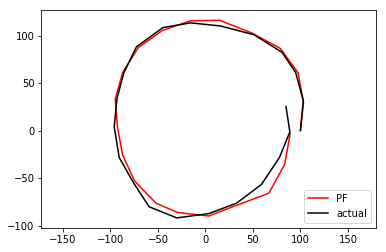
\includegraphics[width=75mm]{report8-3/PF_1/PF1.png}
    \end{center}
    \caption{Particle Filterによる推定}
    \label{pic:PF1}
  \end{minipage}
  \begin{minipage}{0.5\hsize}
    \begin{center}
      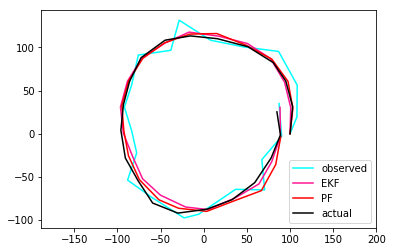
\includegraphics[width=75mm]{report8-3/PF_1/PF2.png}
    \end{center}
    \caption{他の推定法との比較}
    \label{pic:PF2}
  \end{minipage}
\end{figure}
\newpage
\subsection{考察}
上のシミュレーション結果について、それぞれのシミュレーション結果(Figure \ref{pic:PF2})の
平均推定誤差を問題8-2のときと同様に求める。結果は以下のようになった。
\begin{shadebox}
  \begin{verbatim}
  観測による推定値の誤差:20.942228001376662
  EKFによる推定値の誤差:9.459363359394533
  PFによる推定値の誤差:3.88452651804853
  \end{verbatim}
\end{shadebox}
また、100回のシミュレーションを行ったときに、推定値の誤差平均は以下のようになった。

これより、Particleフィルタの方が、EKFよりも精度の良い結果が出ていることがみてとれる。
考えられる要因は以下のとおりである。
\begin{itemize}
  \item ノイズが大きかった。
  \item Particle数が十分大きかった。
\end{itemize}
外乱が大きいことについて、EKFでは、カルマンゲインを求める際に$Q$および$R$の項が
効いてくる、また、非線形のグラフを考えるとヤコビアンによる近似が
行われている。このために、ある程度の誤差が生じる一方で、Particleフィルタでは複数個のサンプリングとその重み
で確率分布の計算が可能である。このため、誤差が大きくても、線形・非線形あるいはグラフの複雑性にかかわらず、
推定精度が高くなると予想される。
次にパーティクル数についてであるが、今回は1000回で行ったがこの値は大きければ大きい方が、
より誤差の少ない値が期待できる。このParticle数による変化をFigure \ref{pic:8-2-2-1}にしめす。誤差がまばらで試行回数も少ないためわかりにくくなって
いるが、誤差はパーティクル数に応じて、微減少していることがわかる。

また、particleフィルターの特徴として、計算が簡易ということが挙げられる。
カルマンフィルター(線形・非線形にかかわらず)は、カルマンゲインを求める際に
は、行列計算を駆使しなければならない。今回はnumpyモジュールを用いたために、
特に困ることはなかったが、より昔の計算機でシミュレーションをしようとなると
かなり複雑になるように思える。また、カルマンフィルタによる推定は観測モデルが
確立されて成り立つが、これも必ずしも利用できるとは言えない。一方で、
Particleフィルタによる推定は、尤度さえ計算できれば、重みの計算も含めて簡単な
計算で構成されている。これもParticleフィルタの期待ができる点といえるのではないだろうか。最後に、
カルマンフィルタでは初めにノイズがガウス分布に乗るという仮定を行ったが、重みさえ計算できれば
よいParticleフィルタではこの仮定は成り立たなくても十分な結果が得られると考えられる。\\
以上より、以下の点でParticleフィルタは優位性が期待できる。
\begin{itemize}
  \item ノイズが大きかったり、ガウス分布に従うとは限らない条件下
  \item 行列計算を行えるような計算機が存在しない、あるいは簡単に期待度の高い
  推定を行いたいとき
  \item 観測モデルが確立されていない条件
\end{itemize}
\begin{figure}[htbp]
  \begin{center}
    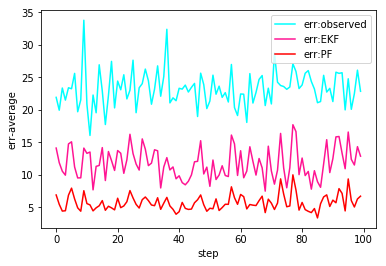
\includegraphics[width=80mm]{report8-3/PF_1/err比較.png}
  \end{center}
  \caption{推定誤差平均の比較(100回)}
\end{figure}
\begin{figure}[htbp]
  \begin{center}
    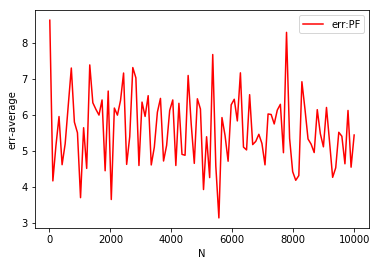
\includegraphics[width=80mm]{report8-3/PF_2/err_trans.png}
    \label{pic:8-2-2-1}
  \end{center}
  \caption{Particke数による推定誤差平均の分布}
\end{figure}
